% =============================================================================
% Section 5: Cross-Axis Structure
% =============================================================================
\section{Cross-Axis Correlation Structure}\label{sec:cross-axis}

This section examines the pairwise linear and rank-order associations
among the six axes.  Strong inter-axis correlations could indicate
redundant information content; near-zero correlations would indicate
that the axes capture genuinely distinct dimensions of strategic
dependence.

\subsection{Pearson and Spearman correlation matrices}

\Cref{tab:corr-pearson} reports the full $6 \times 6$ Pearson
correlation matrix computed on the raw axis scores across
the~27~countries.

\begin{table}[htbp]
\centering
\caption{Pearson correlation matrix of axis-level scores, EU-27,
  2024.  Cells in bold indicate $|r| \geq 0.40$.}
\label{tab:corr-pearson}
\sisetup{table-format=+1.3, tight-spacing}
\begin{tabular}{@{}l
  S S S S S S@{}}
\toprule
 & {\textbf{Fin.}} & {\textbf{Ene.}} & {\textbf{Tec.}}
 & {\textbf{Def.}} & {\textbf{Crit.}} & {\textbf{Log.}} \\
\midrule
Financial       & {1.000} & +0.062 & +0.076 & +0.024 & +0.218 & -0.164 \\
Energy          & +0.062 & {1.000} & \textbf{+0.530} & -0.175 & +0.372 & +0.112 \\
Technology      & +0.076 & \textbf{+0.530} & {1.000} & -0.222 & +0.097 & +0.068 \\
Defence         & +0.024 & -0.175 & -0.222 & {1.000} & +0.191 & +0.286 \\
Critical inputs & +0.218 & +0.372 & +0.097 & +0.191 & {1.000} & \textbf{+0.549} \\
Logistics       & -0.164 & +0.112 & +0.068 & +0.286 & \textbf{+0.549} & {1.000} \\
\bottomrule
\end{tabular}
\end{table}

\Cref{tab:corr-spearman} reports the Spearman rank correlation matrix.
Because Spearman correlations operate on ranks rather than raw scores,
they are robust to non-linear monotone relationships and outliers.

\begin{table}[htbp]
\centering
\caption{Spearman rank correlation matrix of axis-level scores,
  EU-27, 2024.  Cells in bold indicate $|\rho| \geq 0.40$.}
\label{tab:corr-spearman}
\sisetup{table-format=+1.3, tight-spacing}
\begin{tabular}{@{}l
  S S S S S S@{}}
\toprule
 & {\textbf{Fin.}} & {\textbf{Ene.}} & {\textbf{Tec.}}
 & {\textbf{Def.}} & {\textbf{Crit.}} & {\textbf{Log.}} \\
\midrule
Financial       & {1.000} & +0.138 & +0.267 & -0.040 & +0.016 & -0.034 \\
Energy          & +0.138 & {1.000} & \textbf{+0.487} & -0.115 & \textbf{+0.409} & +0.236 \\
Technology      & +0.267 & \textbf{+0.487} & {1.000} & -0.212 & +0.183 & +0.042 \\
Defence         & -0.040 & -0.115 & -0.212 & {1.000} & +0.234 & +0.220 \\
Critical inputs & +0.016 & \textbf{+0.409} & +0.183 & +0.234 & {1.000} & \textbf{+0.545} \\
Logistics       & -0.034 & +0.236 & +0.042 & +0.220 & \textbf{+0.545} & {1.000} \\
\bottomrule
\end{tabular}
\end{table}

\subsection{Interpretation}

Four correlations exceed $|r| = 0.30$ in Pearson terms:

\begin{enumerate}[leftmargin=2em]
  \item \textbf{Critical inputs--Logistics} ($r = 0.549$,
    $\rho = 0.545$).  This is the strongest bivariate association.
    Countries with concentrated critical-material suppliers also tend
    to have concentrated logistics corridors.  This may reflect a
    common exposure to a narrow set of extra-EU partner countries
    (e.g., Turkey, China) that supply both raw materials and transit
    routes.

  \item \textbf{Energy--Technology} ($r = 0.530$, $\rho = 0.487$).
    Countries with high energy-supply concentration tend also to have
    concentrated technology-import patterns.  One plausible channel is
    that smaller EU countries with fewer diversified trade partnerships
    exhibit concentration on both axes simultaneously.

  \item \textbf{Energy--Critical inputs} ($r = 0.372$,
    $\rho = 0.409$).  A moderate positive association, consistent with
    overlapping geographic supply chains for energy commodities and
    critical raw materials.

  \item \textbf{Defence--Logistics} ($r = 0.286$, $\rho = 0.220$).
    A weak-to-moderate positive association.  Countries with
    concentrated defence-import partners also tend to have
    concentrated port/logistics structures, though the relationship is
    not strong.
\end{enumerate}

Several near-zero correlations are equally notable:

\begin{itemize}[leftmargin=2em]
  \item \textbf{Financial--all other axes.}  The financial axis is
    nearly uncorrelated with every other axis ($|r| \leq 0.22$).
    This confirms that the financial axis captures a distinct dimension
    of dependence not captured by trade or physical infrastructure
    measures.

  \item \textbf{Technology--Defence} ($r = -0.222$).  A mild negative
    association, suggesting that countries with diversified technology
    imports may tend toward concentrated defence suppliers, and vice
    versa.
\end{itemize}

\subsection{Correlation heatmap}

\Cref{fig:corr-heatmap} presents a colour-coded heatmap of the
Pearson correlation matrix.

\begin{figure}[htbp]
\centering
% F05: Pearson correlation heatmap (6x6) — hardcoded cells
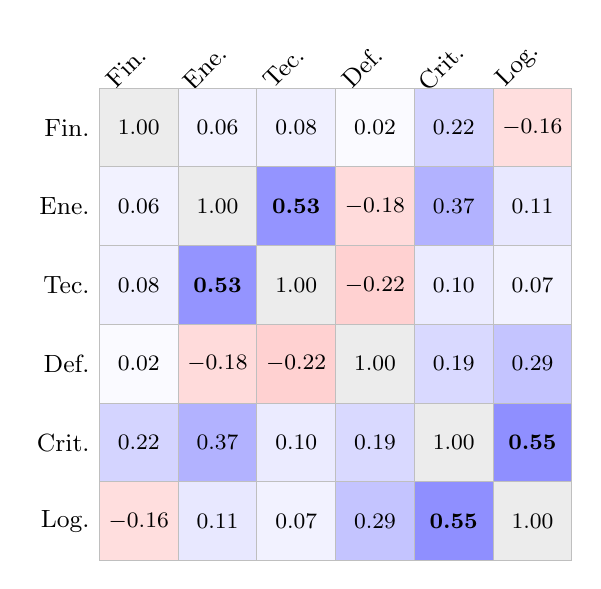
\begin{tikzpicture}
% Axis labels
\def\labels{{"Fin.","Ene.","Tec.","Def.","Crit.","Log."}}
% Row/column labels
\foreach \i in {0,...,5} {
  \pgfmathsetmacro{\lab}{\labels[\i]}
  \node[anchor=east, font=\small] at (0,-\i-0.5) {\lab};
  \node[anchor=south, font=\small, rotate=45] at (\i+0.5,0.1) {\lab};
}
% --- Row 0: Financial ---
\fill[gray!15]   (0, 0) rectangle ++(1,-1); \node[font=\footnotesize] at (0.5,-0.5) {1.00};
\fill[blue!5]    (1, 0) rectangle ++(1,-1); \node[font=\footnotesize] at (1.5,-0.5) {0.06};
\fill[blue!6]    (2, 0) rectangle ++(1,-1); \node[font=\footnotesize] at (2.5,-0.5) {0.08};
\fill[blue!2]    (3, 0) rectangle ++(1,-1); \node[font=\footnotesize] at (3.5,-0.5) {0.02};
\fill[blue!17]   (4, 0) rectangle ++(1,-1); \node[font=\footnotesize] at (4.5,-0.5) {0.22};
\fill[red!13]    (5, 0) rectangle ++(1,-1); \node[font=\footnotesize] at (5.5,-0.5) {$-$0.16};
% --- Row 1: Energy ---
\fill[blue!5]    (0,-1) rectangle ++(1,-1); \node[font=\footnotesize] at (0.5,-1.5) {0.06};
\fill[gray!15]   (1,-1) rectangle ++(1,-1); \node[font=\footnotesize] at (1.5,-1.5) {1.00};
\fill[blue!42]   (2,-1) rectangle ++(1,-1); \node[font=\footnotesize\bfseries] at (2.5,-1.5) {0.53};
\fill[red!14]    (3,-1) rectangle ++(1,-1); \node[font=\footnotesize] at (3.5,-1.5) {$-$0.18};
\fill[blue!30]   (4,-1) rectangle ++(1,-1); \node[font=\footnotesize] at (4.5,-1.5) {0.37};
\fill[blue!9]    (5,-1) rectangle ++(1,-1); \node[font=\footnotesize] at (5.5,-1.5) {0.11};
% --- Row 2: Technology ---
\fill[blue!6]    (0,-2) rectangle ++(1,-1); \node[font=\footnotesize] at (0.5,-2.5) {0.08};
\fill[blue!42]   (1,-2) rectangle ++(1,-1); \node[font=\footnotesize\bfseries] at (1.5,-2.5) {0.53};
\fill[gray!15]   (2,-2) rectangle ++(1,-1); \node[font=\footnotesize] at (2.5,-2.5) {1.00};
\fill[red!18]    (3,-2) rectangle ++(1,-1); \node[font=\footnotesize] at (3.5,-2.5) {$-$0.22};
\fill[blue!8]    (4,-2) rectangle ++(1,-1); \node[font=\footnotesize] at (4.5,-2.5) {0.10};
\fill[blue!5]    (5,-2) rectangle ++(1,-1); \node[font=\footnotesize] at (5.5,-2.5) {0.07};
% --- Row 3: Defence ---
\fill[blue!2]    (0,-3) rectangle ++(1,-1); \node[font=\footnotesize] at (0.5,-3.5) {0.02};
\fill[red!14]    (1,-3) rectangle ++(1,-1); \node[font=\footnotesize] at (1.5,-3.5) {$-$0.18};
\fill[red!18]    (2,-3) rectangle ++(1,-1); \node[font=\footnotesize] at (2.5,-3.5) {$-$0.22};
\fill[gray!15]   (3,-3) rectangle ++(1,-1); \node[font=\footnotesize] at (3.5,-3.5) {1.00};
\fill[blue!15]   (4,-3) rectangle ++(1,-1); \node[font=\footnotesize] at (4.5,-3.5) {0.19};
\fill[blue!23]   (5,-3) rectangle ++(1,-1); \node[font=\footnotesize] at (5.5,-3.5) {0.29};
% --- Row 4: Critical Inputs ---
\fill[blue!17]   (0,-4) rectangle ++(1,-1); \node[font=\footnotesize] at (0.5,-4.5) {0.22};
\fill[blue!30]   (1,-4) rectangle ++(1,-1); \node[font=\footnotesize] at (1.5,-4.5) {0.37};
\fill[blue!8]    (2,-4) rectangle ++(1,-1); \node[font=\footnotesize] at (2.5,-4.5) {0.10};
\fill[blue!15]   (3,-4) rectangle ++(1,-1); \node[font=\footnotesize] at (3.5,-4.5) {0.19};
\fill[gray!15]   (4,-4) rectangle ++(1,-1); \node[font=\footnotesize] at (4.5,-4.5) {1.00};
\fill[blue!44]   (5,-4) rectangle ++(1,-1); \node[font=\footnotesize\bfseries] at (5.5,-4.5) {0.55};
% --- Row 5: Logistics ---
\fill[red!13]    (0,-5) rectangle ++(1,-1); \node[font=\footnotesize] at (0.5,-5.5) {$-$0.16};
\fill[blue!9]    (1,-5) rectangle ++(1,-1); \node[font=\footnotesize] at (1.5,-5.5) {0.11};
\fill[blue!5]    (2,-5) rectangle ++(1,-1); \node[font=\footnotesize] at (2.5,-5.5) {0.07};
\fill[blue!23]   (3,-5) rectangle ++(1,-1); \node[font=\footnotesize] at (3.5,-5.5) {0.29};
\fill[blue!44]   (4,-5) rectangle ++(1,-1); \node[font=\footnotesize\bfseries] at (4.5,-5.5) {0.55};
\fill[gray!15]   (5,-5) rectangle ++(1,-1); \node[font=\footnotesize] at (5.5,-5.5) {1.00};
% Grid lines
\foreach \i in {0,...,5} {
  \foreach \j in {0,...,5} {
    \draw[gray!50, thin] (\j,-\i) rectangle ++(1,-1);
  }
}
\end{tikzpicture}

\caption{Pearson correlation heatmap of the six ISI axes, EU-27,
  2024.  Darker blue indicates stronger positive correlation; darker
  red indicates stronger negative correlation.}
\label{fig:corr-heatmap}
\end{figure}

\subsection{Correlation network graph}

\Cref{fig:corr-network} displays a network graph in which each node
is an axis and edges are drawn for all pairs with $|r| \geq 0.30$.
Edge width is proportional to the absolute correlation.

\begin{figure}[htbp]
\centering
% F06: Correlation network graph (edges for |r| >= 0.30)
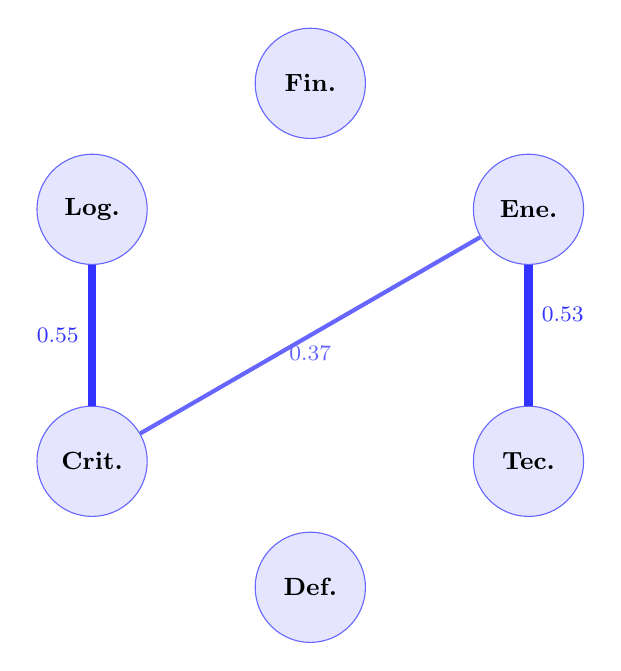
\begin{tikzpicture}[
  node distance=3cm,
  axisnode/.style={circle, draw=blue!60, fill=blue!10,
    minimum size=1.4cm, font=\small\bfseries, align=center},
  edge30/.style={line width=1.5pt, blue!60},
  edge50/.style={line width=3.0pt, blue!80},
]
% Place nodes in a hexagonal layout
\node[axisnode] (fin) at (90:3.2cm)  {Fin.};
\node[axisnode] (ene) at (30:3.2cm)  {Ene.};
\node[axisnode] (tec) at (330:3.2cm) {Tec.};
\node[axisnode] (def) at (270:3.2cm) {Def.};
\node[axisnode] (cri) at (210:3.2cm) {Crit.};
\node[axisnode] (log) at (150:3.2cm) {Log.};

% Edges with |r| >= 0.30
% Energy -- Technology:  r = 0.530
\draw[edge50] (ene) -- (tec) node[midway, above right, font=\footnotesize] {0.53};
% Energy -- Critical:    r = 0.372
\draw[edge30] (ene) -- (cri) node[midway, below, font=\footnotesize] {0.37};
% Critical -- Logistics: r = 0.549
\draw[edge50] (cri) -- (log) node[midway, left, font=\footnotesize] {0.55};
% Note: no other pair exceeds 0.30
\end{tikzpicture}

\caption{Correlation network graph of the six ISI axes.  Edges shown
  for $|r| \geq 0.30$; edge width proportional to~$|r|$.  Three
  edges: energy--technology ($r = 0.53$), energy--critical inputs
  ($r = 0.37$), critical inputs--logistics ($r = 0.55$).}
\label{fig:corr-network}
\end{figure}

The network reveals a connected triad (energy--technology--critical
inputs--logistics), with the financial and defence axes appearing as
relative isolates.  This is consistent with the eigenvalue analysis
below.

\subsection{Eigenvalue structure}

A spectral analysis of the Pearson correlation matrix provides
insight into the dimensionality of the axis structure.

\begin{table}[htbp]
\centering
\caption{Eigenvalues of the $6 \times 6$ Pearson correlation matrix.}
\label{tab:eigenvalues}
\begin{tabular}{@{}lS[table-format=1.4]S[table-format=2.1]S[table-format=2.1]@{}}
\toprule
\textbf{Component} & {\textbf{Eigenvalue}} & {\textbf{\% Var.}}
  & {\textbf{Cum.~\%}} \\
\midrule
PC1 & 1.8996 & 31.7 & 31.7 \\
PC2 & 1.5821 & 26.4 & 58.0 \\
PC3 & 1.0850 & 18.1 & 76.1 \\
PC4 & 0.6674 & 11.1 & 87.2 \\
PC5 & 0.5065 &  8.4 & 95.7 \\
PC6 & 0.2593 &  4.3 & 100.0 \\
\bottomrule
\end{tabular}
\end{table}

Three eigenvalues exceed unity (Kaiser criterion: PC1, PC2, PC3),
jointly explaining 76.1\% of total variance.  The first two principal
components explain 58.0\%.  No single dominant eigenvalue emerges,
confirming that the six axes cannot be collapsed to one or two
dimensions without substantial information loss.

\medskip\noindent\textbf{Implications for composite construction.}
The moderate inter-axis correlations and multi-dimensional eigenvalue
structure support the equal-weight additive aggregation rule
(\cref{eq:composite}): because no single latent factor dominates,
there is no strong empirical basis for differential weighting.
However, the positive critical-inputs--logistics correlation ($r =
0.55$) implies that these two axes partially reinforce each other.
The Dirichlet weight perturbation exercise (\cref{sec:robustness})
provides a direct quantification of the sensitivity of rankings to
alternative weighting schemes.
